% GENERATED FILE - do not hand-edit.
% Source of truth: data/calculus-reviewed/t-3.json in the zenith-website repo.
% Regenerate with: python3 scripts/build_calculus_tex.py
\documentclass[11pt]{article}
\usepackage[utf8]{inputenc}
\usepackage[T1]{fontenc}
\usepackage{amsmath,amssymb}
\usepackage{graphicx}
\usepackage[margin=1in]{geometry}
\graphicspath{{../..//}}
\setlength{\parindent}{0pt}
\setlength{\parskip}{0.6em}
\begin{document}
\section*{Chapter 3: Differentiation --- Test T3}

\bigskip\noindent\textbf{T1.}\ Find $dy/dx$ for $y = x^4 \sec x$.
\begin{list}{}{\setlength{\leftmargin}{3em}\setlength{\labelwidth}{2.5em}\setlength{\itemsep}{0pt}\setlength{\topsep}{2pt}}
\item[(A)] $4x^3 \sec x$
\item[(B)] $4x^3 \sec^2 x$
\item[(C)] $4x^3 + \sec x \tan x$
\item[(D)] $4x^3 \sec x + x^4 \sec x \tan x$
\end{list}

\bigskip\noindent\textbf{T2.}\ Find $dy/dx$ for $y = \dfrac{3-x}{2x+1}$.
\begin{list}{}{\setlength{\leftmargin}{3em}\setlength{\labelwidth}{2.5em}\setlength{\itemsep}{0pt}\setlength{\topsep}{2pt}}
\item[(A)] $-\dfrac{7}{(2x+1)^2}$
\item[(B)] $\dfrac{5-6x}{(2x+1)^2}$
\item[(C)] $-\dfrac{9}{(2x+1)^2}$
\item[(D)] $\dfrac{7}{(2x+1)^2}$
\end{list}

\bigskip\noindent\textbf{T3.}\ Find $dy/dx$ for $y = \sqrt{5-3x}$.
\begin{list}{}{\setlength{\leftmargin}{3em}\setlength{\labelwidth}{2.5em}\setlength{\itemsep}{0pt}\setlength{\topsep}{2pt}}
\item[(A)] $\dfrac{3}{2\sqrt{5-3x}}$
\item[(B)] $-\dfrac{3}{2\sqrt{5-3x}}$
\item[(C)] $-2(5-3x)^{3/2}$
\item[(D)] $2(5-3x)^{3/2}$
\end{list}

\bigskip\noindent\textbf{T4.}\ Find $dy/dx$ for $y = \dfrac{3}{(4x+1)^2}$.
\begin{list}{}{\setlength{\leftmargin}{3em}\setlength{\labelwidth}{2.5em}\setlength{\itemsep}{0pt}\setlength{\topsep}{2pt}}
\item[(A)] $-\dfrac{24}{(4x+1)^2}$
\item[(B)] $-\dfrac{24}{(4x+1)^3}$
\item[(C)] $-\dfrac{6}{(4x+1)^3}$
\item[(D)] $\dfrac{6}{(4x+1)^2}$
\end{list}

\bigskip\noindent\textbf{T5.}\ Find $dy/dx$ for $y = 6x^{2/3} - 8x^{1/2} - 3$.
\begin{list}{}{\setlength{\leftmargin}{3em}\setlength{\labelwidth}{2.5em}\setlength{\itemsep}{0pt}\setlength{\topsep}{2pt}}
\item[(A)] $4x^{-1/3} - 4x^{-1/2}$
\item[(B)] $6x^{-1/3} - 4x^{-1/2}$
\item[(C)] $\dfrac{18}{5}x^{5/3} - \dfrac{16}{3}x^{3/2}$
\item[(D)] $2x^{-1/3} - 2x^{-1/2}$
\end{list}

\bigskip\noindent\textbf{T6.}\ Find $dy/dx$ for $y = 3\sqrt{x} - \dfrac{1}{3\sqrt{x}}$.
\begin{list}{}{\setlength{\leftmargin}{3em}\setlength{\labelwidth}{2.5em}\setlength{\itemsep}{0pt}\setlength{\topsep}{2pt}}
\item[(A)] $\dfrac{9x-1}{6x\sqrt{x}}$
\item[(B)] $\dfrac{9x+1}{6x\sqrt{x}}$
\item[(C)] $\dfrac{3}{\sqrt{x}} + \dfrac{1}{6x\sqrt{x}}$
\item[(D)] $\dfrac{3}{\sqrt{x}} - \dfrac{1}{6x\sqrt{x}}$
\end{list}

\bigskip\noindent\textbf{T7.}\ Find $dy/dx$ for $y = \sqrt{x^2+4x-2}$.
\begin{list}{}{\setlength{\leftmargin}{3em}\setlength{\labelwidth}{2.5em}\setlength{\itemsep}{0pt}\setlength{\topsep}{2pt}}
\item[(A)] $\dfrac{x+2}{y}$
\item[(B)] $2y(x+2)$
\item[(C)] $\dfrac{1}{2\sqrt{x^2+4x-2}}$
\item[(D)] $-\dfrac{x+2}{(x^2+4x-2)^{3/2}}$
\end{list}

\bigskip\noindent\textbf{T8.}\ Find $dy/dx$ for $y = \dfrac{x^3}{\sin x}$.
\begin{list}{}{\setlength{\leftmargin}{3em}\setlength{\labelwidth}{2.5em}\setlength{\itemsep}{0pt}\setlength{\topsep}{2pt}}
\item[(A)] $-\dfrac{3x^2}{\cos x}$
\item[(B)] $\dfrac{3x^2\sin x - x^3\cos x}{\sin^2 x}$
\item[(C)] $\dfrac{3x^2\sin x + x^3\cos x}{\sin^2 x}$
\item[(D)] $\dfrac{3x^2\sin x - x^3\cos x}{\cos^2 x}$
\end{list}

\bigskip\noindent\textbf{T9.}\ Find $dy/dx$ for $y = \ln\!\left(\dfrac{e^x}{e^x+1}\right)$.
\begin{list}{}{\setlength{\leftmargin}{3em}\setlength{\labelwidth}{2.5em}\setlength{\itemsep}{0pt}\setlength{\topsep}{2pt}}
\item[(A)] $x - \dfrac{e^x}{e^x+1}$
\item[(B)] $\dfrac{1}{e^x+1}$
\item[(C)] $-\dfrac{1}{e^x+1}$
\item[(D)] $\dfrac{e^x-2}{e^x+1}$
\end{list}

\bigskip\noindent\textbf{T10.}\ Find $dy/dx$ for $y = \tan^{-1}\dfrac{x}{3}$.
\begin{list}{}{\setlength{\leftmargin}{3em}\setlength{\labelwidth}{2.5em}\setlength{\itemsep}{0pt}\setlength{\topsep}{2pt}}
\item[(A)] $\dfrac{9}{9+x^2}$
\item[(B)] $\dfrac{1}{2\sqrt{9-x^2}}$
\item[(C)] $\dfrac{2}{\sqrt{9-x^2}}$
\item[(D)] $\dfrac{3}{x^2+9}$
\end{list}

\bigskip\noindent\textbf{T11.}\ Find $dy/dx$ for $y = \ln(\csc x + \cot x)$.
\begin{list}{}{\setlength{\leftmargin}{3em}\setlength{\labelwidth}{2.5em}\setlength{\itemsep}{0pt}\setlength{\topsep}{2pt}}
\item[(A)] $\csc x$
\item[(B)] $-\csc x$
\item[(C)] $\dfrac{1}{\csc x + \cot x}$
\item[(D)] $-\dfrac{1}{\csc x + \cot x}$
\end{list}

\bigskip\noindent\textbf{T12.}\ Find $dy/dx$ for $y = \dfrac{e^{2x}-e^{-2x}}{e^{2x}+e^{-2x}}$.
\begin{list}{}{\setlength{\leftmargin}{3em}\setlength{\labelwidth}{2.5em}\setlength{\itemsep}{0pt}\setlength{\topsep}{2pt}}
\item[(A)] $0$
\item[(B)] $2$
\item[(C)] $\dfrac{8}{(e^{2x}+e^{-2x})^2}$
\item[(D)] $\dfrac{1}{e^{4x}+e^{-4x}}$
\end{list}

\bigskip\noindent\textbf{T13.}\ Find $dy/dx$ for $y = \ln\!\left(\sqrt{x^2+4}\right)$.
\begin{list}{}{\setlength{\leftmargin}{3em}\setlength{\labelwidth}{2.5em}\setlength{\itemsep}{0pt}\setlength{\topsep}{2pt}}
\item[(A)] $\dfrac{1}{\sqrt{x^2+4}}$
\item[(B)] $\dfrac{2x}{\sqrt{x^2+4}}$
\item[(C)] $\dfrac{1}{2(x^2+4)}$
\item[(D)] $\dfrac{x}{x^2+4}$
\end{list}

\bigskip\noindent\textbf{T14.}\ Find $dy/dx$ for $y = \sin\!\left(\dfrac{1}{2x}\right)$.
\begin{list}{}{\setlength{\leftmargin}{3em}\setlength{\labelwidth}{2.5em}\setlength{\itemsep}{0pt}\setlength{\topsep}{2pt}}
\item[(A)] $\cos\!\left(\dfrac{1}{2x}\right)$
\item[(B)] $\cos\!\left(-\dfrac{1}{2x^2}\right)$
\item[(C)] $-\dfrac{1}{2x^2}\cos\!\left(\dfrac{1}{2x}\right)$
\item[(D)] $-\dfrac{1}{2x^2}\sin\!\left(\dfrac{1}{2x}\right) + \dfrac{1}{2x}\cos\!\left(\dfrac{1}{2x}\right)$
\end{list}

\bigskip\noindent\textbf{T15.}\ Find $dy/dx$ for $y = \dfrac{1}{3\sin 3x}$.
\begin{list}{}{\setlength{\leftmargin}{3em}\setlength{\labelwidth}{2.5em}\setlength{\itemsep}{0pt}\setlength{\topsep}{2pt}}
\item[(A)] $-\csc 3x \cot 3x$
\item[(B)] $\dfrac{1}{9\cos 3x}$
\item[(C)] $-3\csc 3x \cot 3x$
\item[(D)] $-\csc^2 3x$
\end{list}

\bigskip\noindent\textbf{T16.}\ Find $dy/dx$ for $y = e^{-2x}\cos 3x$.
\begin{list}{}{\setlength{\leftmargin}{3em}\setlength{\labelwidth}{2.5em}\setlength{\itemsep}{0pt}\setlength{\topsep}{2pt}}
\item[(A)] $-e^{-2x}(\cos 3x + 3\sin 3x)$
\item[(B)] $e^{-2x}(\sin 3x - \cos 3x)$
\item[(C)] $3e^{-2x}\sin 3x$
\item[(D)] $-e^{-2x}(2\cos 3x + 3\sin 3x)$
\end{list}

\bigskip\noindent\textbf{T17.}\ Find $dy/dx$ for $y = \cot^2(x)$.
\begin{list}{}{\setlength{\leftmargin}{3em}\setlength{\labelwidth}{2.5em}\setlength{\itemsep}{0pt}\setlength{\topsep}{2pt}}
\item[(A)] $-2\csc x$
\item[(B)] $-2\csc x \cot x$
\item[(C)] $-2\csc^2 x \cot x$
\item[(D)] $\cot x$
\end{list}

\bigskip\noindent\textbf{T18.}\ Find $dy/dx$ for $y = x(\ln x)^2$.
\begin{list}{}{\setlength{\leftmargin}{3em}\setlength{\labelwidth}{2.5em}\setlength{\itemsep}{0pt}\setlength{\topsep}{2pt}}
\item[(A)] $\dfrac{2\ln x}{x}$
\item[(B)] $2\ln x$
\item[(C)] $-2x\ln x + (\ln x)^2$
\item[(D)] $(\ln x)^2 + 2\ln x$
\end{list}

\bigskip\noindent\textbf{T19.}\ Find $dy/dx$ for $y = \dfrac{1-x^2}{1+x^2}$.
\begin{list}{}{\setlength{\leftmargin}{3em}\setlength{\labelwidth}{2.5em}\setlength{\itemsep}{0pt}\setlength{\topsep}{2pt}}
\item[(A)] $-\dfrac{4x}{(1+x^2)^2}$
\item[(B)] $\dfrac{4x}{(1+x^2)^2}$
\item[(C)] $-\dfrac{4x^3}{(1+x^2)^2}$
\item[(D)] $-\dfrac{2x}{1+x^2}$
\end{list}

\bigskip\noindent\textbf{T20.}\ Find $dy/dx$ for $y = \cos^{-1}x + \sqrt{1-x^2}$.
\begin{list}{}{\setlength{\leftmargin}{3em}\setlength{\labelwidth}{2.5em}\setlength{\itemsep}{0pt}\setlength{\topsep}{2pt}}
\item[(A)] $\dfrac{1}{2\sqrt{1-x^2}}$
\item[(B)] $\dfrac{2}{\sqrt{1-x^2}}$
\item[(C)] $-\dfrac{1+x}{\sqrt{1-x^2}}$
\item[(D)] $\dfrac{x^2}{\sqrt{1-x^2}}$
\end{list}

\bigskip\noindent\textbf{T21.}\ Find $dy/dx$ for $2x^3 - 3y^3 = 1$.
\begin{list}{}{\setlength{\leftmargin}{3em}\setlength{\labelwidth}{2.5em}\setlength{\itemsep}{0pt}\setlength{\topsep}{2pt}}
\item[(A)] $x$
\item[(B)] $3x^2$
\item[(C)] $\dfrac{2x^2}{3y^2}$
\item[(D)] $\dfrac{3x^2-1}{y^2}$
\end{list}

\bigskip\noindent\textbf{T22.}\ Find $dy/dx$ for $x + \sin(x+y) = 0$.
\begin{list}{}{\setlength{\leftmargin}{3em}\setlength{\labelwidth}{2.5em}\setlength{\itemsep}{0pt}\setlength{\topsep}{2pt}}
\item[(A)] $\csc(x+y) - 1$
\item[(B)] $\csc(x+y)$
\item[(C)] $-(1+\sec(x+y))$
\item[(D)] $\dfrac{1-\sin x}{\sin y}$
\end{list}

\bigskip\noindent\textbf{T23.}\ Find $dy/dx$ for $\cos x-\sin y-1=0$ at a point where $\cos y\ne0$.
\begin{list}{}{\setlength{\leftmargin}{3em}\setlength{\labelwidth}{2.5em}\setlength{\itemsep}{0pt}\setlength{\topsep}{2pt}}
\item[(A)] $-\cot x$
\item[(B)] $-\sin x \sec y$
\item[(C)] $-\tan x$
\item[(D)] $\dfrac{\sin x}{\cos y}$
\end{list}

\bigskip\noindent\textbf{T24.}\ Find $dy/dx$ for $4x^2 - 3xy + 2y^2 = 1$.
\begin{list}{}{\setlength{\leftmargin}{3em}\setlength{\labelwidth}{2.5em}\setlength{\itemsep}{0pt}\setlength{\topsep}{2pt}}
\item[(A)] $\dfrac{8x-3y}{3x-4y}$
\item[(B)] $\dfrac{3x+y}{x-5y}$
\item[(C)] $3x+5y$
\item[(D)] $\dfrac{3x+4y}{x}$
\end{list}

\bigskip\noindent\textbf{T25.}\ If $x = t^2+2$ and $y = 3t^4$, then $\dfrac{dy}{dx} =$
\begin{list}{}{\setlength{\leftmargin}{3em}\setlength{\labelwidth}{2.5em}\setlength{\itemsep}{0pt}\setlength{\topsep}{2pt}}
\item[(A)] $3t$
\item[(B)] $6t^2$
\item[(C)] $\dfrac{6t^2}{(t^2+2)^2}$
\item[(D)] $\dfrac{6t^4}{(t^2+2)^2}$
\end{list}

\bigskip\noindent\textbf{T26.}\ If $f(x) = x^4 - 8x^3 + 16x^2 - 1$, then the set of values of $x$ for which the derivative equals zero is
\begin{list}{}{\setlength{\leftmargin}{3em}\setlength{\labelwidth}{2.5em}\setlength{\itemsep}{0pt}\setlength{\topsep}{2pt}}
\item[(A)] $\{2,4\}$
\item[(B)] $\{0,-2,-4\}$
\item[(C)] $\{-2,4\}$
\item[(D)] $\{0,2,4\}$
\end{list}

\bigskip\noindent\textbf{T27.}\ If $f(x) = 32\sqrt{x}$, then $f''(4)$ is equal to
\begin{list}{}{\setlength{\leftmargin}{3em}\setlength{\labelwidth}{2.5em}\setlength{\itemsep}{0pt}\setlength{\topsep}{2pt}}
\item[(A)] $-4$
\item[(B)] $-2$
\item[(C)] $-1$
\item[(D)] $-\dfrac{1}{4}$
\end{list}

\bigskip\noindent\textbf{T28.}\ If $f(x) = \ln(x^2)$, then $f''(2)$ is
\begin{list}{}{\setlength{\leftmargin}{3em}\setlength{\labelwidth}{2.5em}\setlength{\itemsep}{0pt}\setlength{\topsep}{2pt}}
\item[(A)] $-\dfrac{1}{4}$
\item[(B)] $-\dfrac{1}{2}$
\item[(C)] $-2$
\item[(D)] $2$
\end{list}

\bigskip\noindent\textbf{T29.}\ If a point moves on the curve $x^2+y^2=169$, then, at $(0,13)$, $\dfrac{d^2y}{dx^2}$ is
\begin{list}{}{\setlength{\leftmargin}{3em}\setlength{\labelwidth}{2.5em}\setlength{\itemsep}{0pt}\setlength{\topsep}{2pt}}
\item[(A)] $0$
\item[(B)] $\dfrac{1}{13}$
\item[(C)] $-13$
\item[(D)] $-\dfrac{1}{13}$
\end{list}

\bigskip\noindent\textbf{T30.}\ If $x = t^2-3$ and $y = t^4-3t^3$, then, when $t=1$, $\dfrac{d^2y}{dx^2}$ is
\begin{list}{}{\setlength{\leftmargin}{3em}\setlength{\labelwidth}{2.5em}\setlength{\itemsep}{0pt}\setlength{\topsep}{2pt}}
\item[(A)] $-\dfrac{1}{4}$
\item[(B)] $\dfrac{1}{4}$
\item[(C)] $-1$
\item[(D)] $1$
\end{list}

\bigskip\noindent\textbf{T31.}\ If $f(x) = 4^x$ and $4^{1.002} \approx 4.011$, which is closest to $f'(1)$?
\begin{list}{}{\setlength{\leftmargin}{3em}\setlength{\labelwidth}{2.5em}\setlength{\itemsep}{0pt}\setlength{\topsep}{2pt}}
\item[(A)] $0.011$
\item[(B)] $4.0$
\item[(C)] $5.5$
\item[(D)] $16.0$
\end{list}

\bigskip\noindent\textbf{T32.}\ If $y = e^x(x-3)$, then $y''(0)$ equals
\begin{list}{}{\setlength{\leftmargin}{3em}\setlength{\labelwidth}{2.5em}\setlength{\itemsep}{0pt}\setlength{\topsep}{2pt}}
\item[(A)] $-2$
\item[(B)] $-1$
\item[(C)] $1$
\item[(D)] $e$
\end{list}

\bigskip\noindent\textbf{T33.}\ If $x = e^\theta \sin\theta$ and $y = e^\theta \cos\theta$, then, when $\theta = \dfrac{\pi}{2}$, $\dfrac{dy}{dx}$ is
\begin{list}{}{\setlength{\leftmargin}{3em}\setlength{\labelwidth}{2.5em}\setlength{\itemsep}{0pt}\setlength{\topsep}{2pt}}
\item[(A)] $1$
\item[(B)] $0$
\item[(C)] $e^{\pi/2}$
\item[(D)] $-1$
\end{list}

\bigskip\noindent\textbf{T34.}\ Given $x = \sin t$ and $y = \cos 2t$, if $\cos(t) \neq 0$, then $\dfrac{d^2y}{dx^2}$ is
\begin{list}{}{\setlength{\leftmargin}{3em}\setlength{\labelwidth}{2.5em}\setlength{\itemsep}{0pt}\setlength{\topsep}{2pt}}
\item[(A)] $4\cos t$
\item[(B)] $4$
\item[(C)] $-4$
\item[(D)] $-4\tan t$
\end{list}

\bigskip\noindent\textbf{T35.}\ $\displaystyle\lim_{h\to 0}\dfrac{(1+h)^4-1}{h}$ is
\begin{list}{}{\setlength{\leftmargin}{3em}\setlength{\labelwidth}{2.5em}\setlength{\itemsep}{0pt}\setlength{\topsep}{2pt}}
\item[(A)] $0$
\item[(B)] $1$
\item[(C)] $4$
\item[(D)] nonexistent
\end{list}

\bigskip\noindent\textbf{T36.}\ $\displaystyle\lim_{h\to 0}\dfrac{\sqrt[3]{27+h}-3}{h}$ is
\begin{list}{}{\setlength{\leftmargin}{3em}\setlength{\labelwidth}{2.5em}\setlength{\itemsep}{0pt}\setlength{\topsep}{2pt}}
\item[(A)] $0$
\item[(B)] $\dfrac{1}{27}$
\item[(C)] $1$
\item[(D)] $243$
\end{list}

\bigskip\noindent\textbf{T37.}\ $\displaystyle\lim_{h\to 0}\dfrac{\ln(e^2+h)-2}{h}$ is
\begin{list}{}{\setlength{\leftmargin}{3em}\setlength{\labelwidth}{2.5em}\setlength{\itemsep}{0pt}\setlength{\topsep}{2pt}}
\item[(A)] $0$
\item[(B)] $\dfrac{1}{e^2}$
\item[(C)] $1$
\item[(D)] $e^2$
\end{list}

\bigskip\noindent\textbf{T38.}\ $\displaystyle\lim_{x\to 0}\dfrac{\cos\left(\frac{\pi}{3}+x\right)-\frac{1}{2}}{x}$ is
\begin{list}{}{\setlength{\leftmargin}{3em}\setlength{\labelwidth}{2.5em}\setlength{\itemsep}{0pt}\setlength{\topsep}{2pt}}
\item[(A)] $-\dfrac{\sqrt{3}}{2}$
\item[(B)] $0$
\item[(C)] $\dfrac{1}{2}$
\item[(D)] $\infty$
\end{list}

\bigskip\noindent\textbf{T39.}\ If $f(x) = \begin{cases} \dfrac{9x^2-9}{x-1}, & x \neq 1 \\ 9, & x=1 \end{cases}$, which of the following statements is (are) true?

I. $\displaystyle\lim_{x\to 1} f(x)$ exists
II. $f$ is continuous at $x=1$
III. $f$ is differentiable at $x=1$
\begin{list}{}{\setlength{\leftmargin}{3em}\setlength{\labelwidth}{2.5em}\setlength{\itemsep}{0pt}\setlength{\topsep}{2pt}}
\item[(A)] none
\item[(B)] I only
\item[(C)] I and II only
\item[(D)] I, II, and III
\end{list}

\bigskip\noindent\textbf{T40.}\ If $g(x) = \begin{cases} x^2, & x \leq 2 \\ 4x-4, & x>2 \end{cases}$, which of the following statements is (are) true?

I. $\displaystyle\lim_{x\to 2} g(x)$ exists
II. $g$ is continuous at $x=2$
III. $g$ is differentiable at $x=2$
\begin{list}{}{\setlength{\leftmargin}{3em}\setlength{\labelwidth}{2.5em}\setlength{\itemsep}{0pt}\setlength{\topsep}{2pt}}
\item[(A)] I only
\item[(B)] II only
\item[(C)] I and II only
\item[(D)] I, II, and III
\end{list}

\bigskip\noindent\textbf{T41.}\ The function $f(x) = x^{4/5}$ on $[-32,32]$ does not satisfy the conditions of the Mean Value Theorem because
\begin{list}{}{\setlength{\leftmargin}{3em}\setlength{\labelwidth}{2.5em}\setlength{\itemsep}{0pt}\setlength{\topsep}{2pt}}
\item[(A)] $f(0)$ is not defined
\item[(B)] $f(x)$ is not continuous on $[-32,32]$
\item[(C)] $f(x)$ is not defined for $x<0$
\item[(D)] $f'(0)$ does not exist
\end{list}

\bigskip\noindent\textbf{T42.}\ If $f(x) = 3x^3-9x$, at what point on the interval $0 \leq x \leq \sqrt{3}$, if any, is the tangent to the curve parallel to the secant line on that interval?
\begin{list}{}{\setlength{\leftmargin}{3em}\setlength{\labelwidth}{2.5em}\setlength{\itemsep}{0pt}\setlength{\topsep}{2pt}}
\item[(A)] $1$
\item[(B)] $\sqrt{2}$
\item[(C)] $0$
\item[(D)] nowhere
\end{list}

\bigskip\noindent\textbf{T43.}\ If $h$ is the inverse function of $f$ and if $f(x) = \dfrac{1}{x}$, then $h'(5) =$
\begin{list}{}{\setlength{\leftmargin}{3em}\setlength{\labelwidth}{2.5em}\setlength{\itemsep}{0pt}\setlength{\topsep}{2pt}}
\item[(A)] $-25$
\item[(B)] $-\dfrac{1}{25}$
\item[(C)] $\dfrac{1}{25}$
\item[(D)] $25$
\end{list}

\bigskip\noindent\textbf{T44.}\ $\displaystyle\lim_{x\to\infty}\dfrac{e^x}{x^{30}}$ equals
\begin{list}{}{\setlength{\leftmargin}{3em}\setlength{\labelwidth}{2.5em}\setlength{\itemsep}{0pt}\setlength{\topsep}{2pt}}
\item[(A)] $0$
\item[(B)] $1$
\item[(C)] $\dfrac{1}{30!}$
\item[(D)] $\infty$
\end{list}

\bigskip\noindent\textbf{T45.}\ If $\cos(xy) = x$, then $\dfrac{dy}{dx} =$
\begin{list}{}{\setlength{\leftmargin}{3em}\setlength{\labelwidth}{2.5em}\setlength{\itemsep}{0pt}\setlength{\topsep}{2pt}}
\item[(A)] $-\dfrac{\csc(xy)}{x}$
\item[(B)] $-\dfrac{\csc(xy)+y}{x}$
\item[(C)] $\dfrac{1-\csc(xy)}{x}$
\item[(D)] $-\csc(xy) - 1$
\end{list}

\bigskip\noindent\textbf{T46.}\ $\displaystyle\lim_{x\to 0}\dfrac{\sin 3x}{x}$ is
\begin{list}{}{\setlength{\leftmargin}{3em}\setlength{\labelwidth}{2.5em}\setlength{\itemsep}{0pt}\setlength{\topsep}{2pt}}
\item[(A)] $1$
\item[(B)] $3$
\item[(C)] $\dfrac{1}{3}$
\item[(D)] $0$
\end{list}

\bigskip\noindent\textbf{T47.}\ $\displaystyle\lim_{x\to 0}\dfrac{\sin 2x}{\sin 5x}$ is
\begin{list}{}{\setlength{\leftmargin}{3em}\setlength{\labelwidth}{2.5em}\setlength{\itemsep}{0pt}\setlength{\topsep}{2pt}}
\item[(A)] $1$
\item[(B)] $\dfrac{5}{2}$
\item[(C)] $\dfrac{2}{5}$
\item[(D)] $0$
\end{list}

\bigskip\noindent\textbf{T48.}\ $\displaystyle\lim_{x\to 0}\dfrac{1-\cos 5x}{x}$ is
\begin{list}{}{\setlength{\leftmargin}{3em}\setlength{\labelwidth}{2.5em}\setlength{\itemsep}{0pt}\setlength{\topsep}{2pt}}
\item[(A)] $0$
\item[(B)] $1$
\item[(C)] $2$
\item[(D)] $\infty$
\end{list}

\bigskip\noindent\textbf{T49.}\ $\displaystyle\lim_{x\to 0}\dfrac{\tan 2\pi x}{x}$ is
\begin{list}{}{\setlength{\leftmargin}{3em}\setlength{\labelwidth}{2.5em}\setlength{\itemsep}{0pt}\setlength{\topsep}{2pt}}
\item[(A)] $0$
\item[(B)] $1$
\item[(C)] $2\pi$
\item[(D)] $\infty$
\end{list}

\bigskip\noindent\textbf{T50.}\ $\displaystyle\lim_{x\to\infty} x^3 \sin\dfrac{1}{x^2}$
\begin{list}{}{\setlength{\leftmargin}{3em}\setlength{\labelwidth}{2.5em}\setlength{\itemsep}{0pt}\setlength{\topsep}{2pt}}
\item[(A)] is $1$
\item[(B)] is $0$
\item[(C)] is $\infty$
\item[(D)] oscillates between $-1$ and $1$
\end{list}

\bigskip\noindent\textbf{T51.}\ The graph in the $xy$-plane represented by $x = 4+3\sin t$ and $y = 3\cos t - 2$, for $-\pi \leq t \leq \pi$, is
\begin{list}{}{\setlength{\leftmargin}{3em}\setlength{\labelwidth}{2.5em}\setlength{\itemsep}{0pt}\setlength{\topsep}{2pt}}
\item[(A)] a semicircle
\item[(B)] a circle
\item[(C)] an ellipse
\item[(D)] half of an ellipse
\end{list}

\bigskip\noindent\textbf{T52.}\ $\displaystyle\lim_{x\to 0}\dfrac{\sec 2x - \cos 2x}{x^2}$
\begin{list}{}{\setlength{\leftmargin}{3em}\setlength{\labelwidth}{2.5em}\setlength{\itemsep}{0pt}\setlength{\topsep}{2pt}}
\item[(A)] $=0$
\item[(B)] $=1$
\item[(C)] $=2$
\item[(D)] $=4$
\end{list}

\bigskip\noindent\textbf{T53.}\ Find $dy/dx$ for $x = 2t - \sin 2t$ and $y = 1 - \cos 2t$.
\begin{list}{}{\setlength{\leftmargin}{3em}\setlength{\labelwidth}{2.5em}\setlength{\itemsep}{0pt}\setlength{\topsep}{2pt}}
\item[(A)] $\dfrac{\sin 2t}{1-\cos 2t}$
\item[(B)] $\dfrac{1-\cos 2t}{\sin 2t}$
\item[(C)] $\dfrac{\sin 2t}{\cos 2t - 1}$
\item[(D)] $\dfrac{1-x}{y}$
\end{list}

\bigskip\noindent\textbf{T54.}\ Find $dy/dx$ for $x = \sin^3\theta$ and $y = \cos^3\theta$.
\begin{list}{}{\setlength{\leftmargin}{3em}\setlength{\labelwidth}{2.5em}\setlength{\itemsep}{0pt}\setlength{\topsep}{2pt}}
\item[(A)] $-\cot\theta$
\item[(B)] $\cot\theta$
\item[(C)] $-\tan\theta$
\item[(D)] $-\tan^2\theta$
\end{list}

\bigskip\noindent\textbf{T55.}\ Find $dy/dx$ for $x = 1-e^{-2t}$ and $y = t+e^{-2t}$.
\begin{list}{}{\setlength{\leftmargin}{3em}\setlength{\labelwidth}{2.5em}\setlength{\itemsep}{0pt}\setlength{\topsep}{2pt}}
\item[(A)] $\dfrac{e^{-2}}{1-e^{-2t}}$
\item[(B)] $e^{2t}+1$
\item[(C)] $e^{2t}-e^{-4t}$
\item[(D)] $\dfrac{e^{2t}}{2}-1$
\end{list}

\bigskip\noindent\textbf{T56.}\ Find $dy/dx$ for $x = \dfrac{1}{1-2t}$ and $y = 1-\ln(1-2t)$ $(t<\tfrac{1}{2})$.
\begin{list}{}{\setlength{\leftmargin}{3em}\setlength{\labelwidth}{2.5em}\setlength{\itemsep}{0pt}\setlength{\topsep}{2pt}}
\item[(A)] $\dfrac{1}{1-2t}$
\item[(B)] $2t-1$
\item[(C)] $\dfrac{1}{x}$
\item[(D)] $\dfrac{(1-2t)^2}{t}$
\end{list}

\bigskip\noindent\textbf{T57.}\ The ``left half'' of the parabola defined by $y = x^2-10x+24$ for $x \leq 5$ is a one-to-one function; therefore, its inverse is also a function. Call that inverse $g$. Find $g'(3)$.
\begin{list}{}{\setlength{\leftmargin}{3em}\setlength{\labelwidth}{2.5em}\setlength{\itemsep}{0pt}\setlength{\topsep}{2pt}}
\item[(A)] $-\dfrac{1}{2}$
\item[(B)] $-\dfrac{1}{4}$
\item[(C)] $\dfrac{1}{4}$
\item[(D)] $\dfrac{1}{2}$
\end{list}

\bigskip\noindent\textbf{T58.}\ If $f(u) = \sin u$ and $u = g(x) = x^2-16$, then $(f \circ g)'(4)$ equals
\begin{list}{}{\setlength{\leftmargin}{3em}\setlength{\labelwidth}{2.5em}\setlength{\itemsep}{0pt}\setlength{\topsep}{2pt}}
\item[(A)] $0$
\item[(B)] $2$
\item[(C)] $4$
\item[(D)] $8$
\end{list}

\bigskip\noindent\textbf{T59.}\ If $f(x) = \dfrac{x}{(x-2)^2}$, then the set of $x$'s for which $f'(x)$ exists is
\begin{list}{}{\setlength{\leftmargin}{3em}\setlength{\labelwidth}{2.5em}\setlength{\itemsep}{0pt}\setlength{\topsep}{2pt}}
\item[(A)] all reals
\item[(B)] all reals except $x=2$ and $x=-2$
\item[(C)] all reals except $x=-2$
\item[(D)] all reals except $x=2$
\end{list}

\bigskip\noindent\textbf{T60.}\ If $f(x) = \dfrac{1}{x^2+4}$ and $g(x) = \sqrt{x}$, then the derivative of $f(g(x))$ is
\begin{list}{}{\setlength{\leftmargin}{3em}\setlength{\labelwidth}{2.5em}\setlength{\itemsep}{0pt}\setlength{\topsep}{2pt}}
\item[(A)] $-(x+4)^{-2}$
\item[(B)] $-\dfrac{2x}{(x^2+4)^2}$
\item[(C)] $\dfrac{1}{(x+4)^2}$
\item[(D)] $\dfrac{1}{2\sqrt{x}(x+4)}$
\end{list}

\bigskip\noindent\textbf{T61.}\ Let $f(x)=3x^3-4x$ restricted to $x<-2/3$, and let $h$ be its inverse. Find $h\prime(1)$.
\begin{list}{}{\setlength{\leftmargin}{3em}\setlength{\labelwidth}{2.5em}\setlength{\itemsep}{0pt}\setlength{\topsep}{2pt}}
\item[(A)] $-1$
\item[(B)] $\dfrac{1}{5}$
\item[(C)] $1$
\item[(D)] $5$
\end{list}

\bigskip\noindent\textbf{T62.}\ If $f(x) = x^3-4x^2+9x+3$ and $g(x) = f^{-1}(x)$, then $g'(3) =$
\begin{list}{}{\setlength{\leftmargin}{3em}\setlength{\labelwidth}{2.5em}\setlength{\itemsep}{0pt}\setlength{\topsep}{2pt}}
\item[(A)] $9$
\item[(B)] $\dfrac{1}{9}$
\item[(C)] $\dfrac{1}{73}$
\item[(D)] $73$
\end{list}

\bigskip\noindent\textbf{TB1.}\ Differentiable functions $f,g$ have values $\begin{array}{c|rrrr}x&f(x)&f\prime(x)&g(x)&g\prime(x)\\0&3&2&6&-5\\1&5&3&3&-4\\2&8&4&2&-3\\3&14&5&1&-2\end{array}$. If $A(x) = f(x) + 2g(x)$, then $A'(3) =$
\begin{list}{}{\setlength{\leftmargin}{3em}\setlength{\labelwidth}{2.5em}\setlength{\itemsep}{0pt}\setlength{\topsep}{2pt}}
\item[(A)] $-3$
\item[(B)] $1$
\item[(C)] $9$
\item[(D)] $13$
\end{list}

\bigskip\noindent\textbf{TB2.}\ Differentiable functions $f,g$ have values $\begin{array}{c|rrrr}x&f(x)&f\prime(x)&g(x)&g\prime(x)\\0&3&2&6&-5\\1&5&3&3&-4\\2&8&4&2&-3\\3&14&5&1&-2\end{array}$. If $B(x) = f(x) \cdot g(x)$, then $B'(2) =$
\begin{list}{}{\setlength{\leftmargin}{3em}\setlength{\labelwidth}{2.5em}\setlength{\itemsep}{0pt}\setlength{\topsep}{2pt}}
\item[(A)] $-24$
\item[(B)] $-16$
\item[(C)] $-8$
\item[(D)] $16$
\end{list}

\bigskip\noindent\textbf{TB3.}\ Differentiable functions $f,g$ have values $\begin{array}{c|rrrr}x&f(x)&f\prime(x)&g(x)&g\prime(x)\\0&3&2&6&-5\\1&5&3&3&-4\\2&8&4&2&-3\\3&14&5&1&-2\end{array}$. If $D(x) = \dfrac{1}{g(x)}$, then $D'(1) =$
\begin{list}{}{\setlength{\leftmargin}{3em}\setlength{\labelwidth}{2.5em}\setlength{\itemsep}{0pt}\setlength{\topsep}{2pt}}
\item[(A)] $-\dfrac{4}{9}$
\item[(B)] $-\dfrac{1}{9}$
\item[(C)] $\dfrac{1}{9}$
\item[(D)] $\dfrac{4}{9}$
\end{list}

\bigskip\noindent\textbf{TB4.}\ Differentiable functions $f,g$ have values $\begin{array}{c|rrrr}x&f(x)&f\prime(x)&g(x)&g\prime(x)\\0&3&2&6&-5\\1&5&3&3&-4\\2&8&4&2&-3\\3&14&5&1&-2\end{array}$. If $H(x) = \sqrt{f(x)}$, then $H'(3) =$
\begin{list}{}{\setlength{\leftmargin}{3em}\setlength{\labelwidth}{2.5em}\setlength{\itemsep}{0pt}\setlength{\topsep}{2pt}}
\item[(A)] $\dfrac{1}{2\sqrt{14}}$
\item[(B)] $\dfrac{5}{2\sqrt{14}}$
\item[(C)] $\dfrac{5}{\sqrt{14}}$
\item[(D)] $10\sqrt{14}$
\end{list}

\bigskip\noindent\textbf{TB5.}\ Differentiable functions $f,g$ have values $\begin{array}{c|rrrr}x&f(x)&f\prime(x)&g(x)&g\prime(x)\\0&3&2&6&-5\\1&5&3&3&-4\\2&8&4&2&-3\\3&14&5&1&-2\end{array}$. If $K(x) = \dfrac{f(x)}{g(x)}$, then $K'(0) =$
\begin{list}{}{\setlength{\leftmargin}{3em}\setlength{\labelwidth}{2.5em}\setlength{\itemsep}{0pt}\setlength{\topsep}{2pt}}
\item[(A)] $-\dfrac{3}{4}$
\item[(B)] $-\dfrac{9}{25}$
\item[(C)] $\dfrac{3}{4}$
\item[(D)] $\dfrac{9}{16}$
\end{list}

\bigskip\noindent\textbf{TB6.}\ Differentiable functions $f,g$ have values $\begin{array}{c|rrrr}x&f(x)&f\prime(x)&g(x)&g\prime(x)\\0&3&2&6&-5\\1&5&3&3&-4\\2&8&4&2&-3\\3&14&5&1&-2\end{array}$. If $M(x) = f(g(x))$, then $M'(1) =$
\begin{list}{}{\setlength{\leftmargin}{3em}\setlength{\labelwidth}{2.5em}\setlength{\itemsep}{0pt}\setlength{\topsep}{2pt}}
\item[(A)] $-20$
\item[(B)] $-15$
\item[(C)] $15$
\item[(D)] $20$
\end{list}

\bigskip\noindent\textbf{TB7.}\ Differentiable functions $f,g$ have values $\begin{array}{c|rrrr}x&f(x)&f\prime(x)&g(x)&g\prime(x)\\0&3&2&6&-5\\1&5&3&3&-4\\2&8&4&2&-3\\3&14&5&1&-2\end{array}$. If $P(x) = f(x^3)$, then $P'(1) =$
\begin{list}{}{\setlength{\leftmargin}{3em}\setlength{\labelwidth}{2.5em}\setlength{\itemsep}{0pt}\setlength{\topsep}{2pt}}
\item[(A)] $3$
\item[(B)] $6$
\item[(C)] $9$
\item[(D)] $15$
\end{list}

\bigskip\noindent\textbf{TB8.}\ Differentiable functions $f,g$ have values $\begin{array}{c|rrrr}x&f(x)&f\prime(x)&g(x)&g\prime(x)\\0&3&2&6&-5\\1&5&3&3&-4\\2&8&4&2&-3\\3&14&5&1&-2\end{array}$. If $S(x) = f^{-1}(x)$, then $S'(3) =$
\begin{list}{}{\setlength{\leftmargin}{3em}\setlength{\labelwidth}{2.5em}\setlength{\itemsep}{0pt}\setlength{\topsep}{2pt}}
\item[(A)] $-2$
\item[(B)] $\dfrac{1}{4}$
\item[(C)] $\dfrac{1}{2}$
\item[(D)] $2$
\end{list}

\bigskip\noindent\textbf{TB9.}\ The graph of $g'$ is shown here. Which of the following statements is (are) true of $g$?

I. $g$ is continuous at $x=a$
II. $g$ is differentiable at $x=a$
III. $g$ is increasing in an interval containing $x=a$
\begin{center}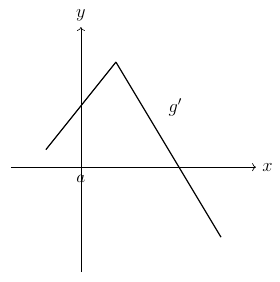
\includegraphics[width=0.6\linewidth]{data/calculus-figures/t3-b9.png}\end{center}
\begin{list}{}{\setlength{\leftmargin}{3em}\setlength{\labelwidth}{2.5em}\setlength{\itemsep}{0pt}\setlength{\topsep}{2pt}}
\item[(A)] I only
\item[(B)] III only
\item[(C)] I and III only
\item[(D)] I, II, and III
\end{list}

\bigskip\noindent\textbf{TB10.}\ The figure gives $f\prime$ on either side of $x=a$, but supplies no value for $f(a)$. Which conclusion is justified?
\begin{center}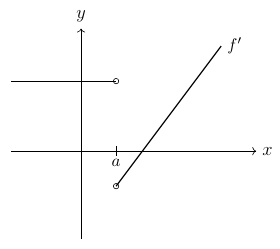
\includegraphics[width=0.6\linewidth]{data/calculus-figures/t3-b10.png}\end{center}
\begin{list}{}{\setlength{\leftmargin}{3em}\setlength{\labelwidth}{2.5em}\setlength{\itemsep}{0pt}\setlength{\topsep}{2pt}}
\item[(A)] The information does not determine whether $f$ is continuous at $x=a$.
\item[(B)] $f$ has a vertical asymptote at $x=a$
\item[(C)] $f$ has a jump discontinuity at $x=a$
\item[(D)] $f$ has a removable discontinuity at $x=a$
\end{list}

\bigskip\noindent\textbf{TB11.}\ The function $f$ whose graph is shown has $f'=0$ at $x=$
\begin{center}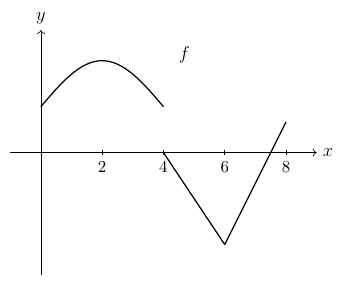
\includegraphics[width=0.6\linewidth]{data/calculus-figures/t3-b11.png}\end{center}
\begin{list}{}{\setlength{\leftmargin}{3em}\setlength{\labelwidth}{2.5em}\setlength{\itemsep}{0pt}\setlength{\topsep}{2pt}}
\item[(A)] $2$ only
\item[(B)] $2$ and $6$
\item[(C)] $6$ and $8$
\item[(D)] $2$, $6$, and $8$
\end{list}

\bigskip\noindent\textbf{TB12.}\ A differentiable function $f$ has the values shown. Estimate $f'(1.5)$.

\[\begin{array}{|c|c|c|c|c|}
\hline
x & 1.0 & 1.3 & 1.4 & 1.6 \\
\hline
f(x) & 6 & 8 & 12 & 24 \\
\hline
\end{array}\]
\begin{list}{}{\setlength{\leftmargin}{3em}\setlength{\labelwidth}{2.5em}\setlength{\itemsep}{0pt}\setlength{\topsep}{2pt}}
\item[(A)] $8$
\item[(B)] $24$
\item[(C)] $60$
\item[(D)] $120$
\end{list}

\bigskip\noindent\textbf{TB13.}\ The conical reservoir has its vertex at the bottom. Water is poured into a conical reservoir at a constant rate. If $h(t)$ is the rate of change of the depth of the water, then $h$ is
\begin{list}{}{\setlength{\leftmargin}{3em}\setlength{\labelwidth}{2.5em}\setlength{\itemsep}{0pt}\setlength{\topsep}{2pt}}
\item[(A)] linear and increasing
\item[(B)] linear and decreasing
\item[(C)] nonlinear and increasing
\item[(D)] nonlinear and decreasing
\end{list}

\bigskip\noindent\textbf{TB14.}\ Use the graph below, consisting of two line segments and a lower semicircle of radius $3$. $f'(x) = 0$ for $x =$
\begin{center}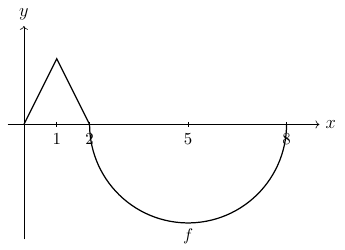
\includegraphics[width=0.6\linewidth]{data/calculus-figures/t3-b14-b16.png}\end{center}
\begin{list}{}{\setlength{\leftmargin}{3em}\setlength{\labelwidth}{2.5em}\setlength{\itemsep}{0pt}\setlength{\topsep}{2pt}}
\item[(A)] $1$ only
\item[(B)] $2$ only
\item[(C)] $5$ only
\item[(D)] $1$ and $5$
\end{list}

\bigskip\noindent\textbf{TB15.}\ Use the graph below, consisting of two line segments and a lower semicircle of radius $3$. For $0 < x < 8$, $f'(x)$ does not exist for $x =$
\begin{center}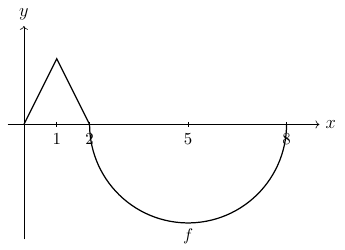
\includegraphics[width=0.6\linewidth]{data/calculus-figures/t3-b14-b16.png}\end{center}
\begin{list}{}{\setlength{\leftmargin}{3em}\setlength{\labelwidth}{2.5em}\setlength{\itemsep}{0pt}\setlength{\topsep}{2pt}}
\item[(A)] $1$ only
\item[(B)] $2$ only
\item[(C)] $1$ and $2$
\item[(D)] $2$ and $8$
\end{list}

\bigskip\noindent\textbf{TB16.}\ Use the graph below, consisting of two line segments and a lower semicircle of radius $3$. $f'(7) =$
\begin{center}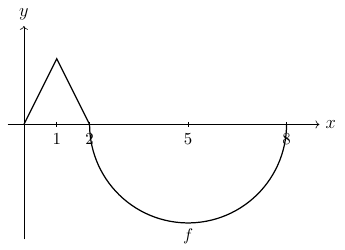
\includegraphics[width=0.6\linewidth]{data/calculus-figures/t3-b14-b16.png}\end{center}
\begin{list}{}{\setlength{\leftmargin}{3em}\setlength{\labelwidth}{2.5em}\setlength{\itemsep}{0pt}\setlength{\topsep}{2pt}}
\item[(A)] $\dfrac{1}{2}$
\item[(B)] $\dfrac{1}{\sqrt{5}}$
\item[(C)] $\dfrac{2}{\sqrt{5}}$
\item[(D)] $\sqrt{5}$
\end{list}

\bigskip\noindent\textbf{TB17.}\ At how many points on the interval $[-6,6]$ is a tangent to $y = x + \sin x$ parallel to the secant line on $[-6,6]$?
\begin{list}{}{\setlength{\leftmargin}{3em}\setlength{\labelwidth}{2.5em}\setlength{\itemsep}{0pt}\setlength{\topsep}{2pt}}
\item[(A)] none
\item[(B)] $2$
\item[(C)] $3$
\item[(D)] $4$
\end{list}

\bigskip\noindent\textbf{TB18.}\ From the values of $f$ shown, estimate $f'(3)$.

\[\begin{array}{|c|c|c|c|c|c|}
\hline
x & 2.90 & 2.95 & 2.97 & 2.99 & 3.00 \\
\hline
f(x) & 9.00 & 7.00 & 6.20 & 6.02 & 6.00 \\
\hline
\end{array}\]
\begin{list}{}{\setlength{\leftmargin}{3em}\setlength{\labelwidth}{2.5em}\setlength{\itemsep}{0pt}\setlength{\topsep}{2pt}}
\item[(A)] $-0.10$
\item[(B)] $-0.20$
\item[(C)] $-2$
\item[(D)] $-10$
\end{list}

\bigskip\noindent\textbf{TB19.}\ Given $f(2.99)=6.02$ and $f(3)=6.00$, estimate $(f^{-1})\prime(6)$.
\begin{list}{}{\setlength{\leftmargin}{3em}\setlength{\labelwidth}{2.5em}\setlength{\itemsep}{0pt}\setlength{\topsep}{2pt}}
\item[(A)] $-0.5$
\item[(B)] $-0.2$
\item[(C)] $-2$
\item[(D)] $-5$
\end{list}

\bigskip\noindent\textbf{TB20.}\ The table below shows some points on a function $f$ that is both continuous and differentiable on the closed interval $[2,10]$.

\[\begin{array}{|c|c|c|c|c|c|}
\hline
x & 2 & 4 & 6 & 8 & 10 \\
\hline
f(x) & 40 & 32 & 28 & 32 & 40 \\
\hline
\end{array}\]

Which must be true?
\begin{list}{}{\setlength{\leftmargin}{3em}\setlength{\labelwidth}{2.5em}\setlength{\itemsep}{0pt}\setlength{\topsep}{2pt}}
\item[(A)] $f'(6) = 0$
\item[(B)] $f'(8) > 0$
\item[(C)] The maximum value of $f$ on the interval $[2,10]$ is $40$.
\item[(D)] For some value of $x$ on the interval $[2,10]$, $f'(x) = 0$.
\end{list}

\bigskip\noindent\textbf{TB21.}\ Let $f$ be twice continuously differentiable on $\mathbb R$. Suppose $[f(a+h)-f(a)]/h\ge f\prime(a)$ for every real $a$ and every $h>0$. Which statement must hold?
\begin{list}{}{\setlength{\leftmargin}{3em}\setlength{\labelwidth}{2.5em}\setlength{\itemsep}{0pt}\setlength{\topsep}{2pt}}
\item[(A)] $f\prime(x)\ge0$ for all real $x$
\item[(B)] $f\prime(x)\le0$ for all real $x$
\item[(C)] $f\prime\prime(x)\ge0$ for all real $x$
\item[(D)] $f\prime\prime(x)\le0$ for all real $x$
\end{list}

\bigskip\noindent\textbf{TB22.}\ If $f(a) = f(b) = 0$ and $f(x)$ is continuous on $[a,b]$, then
\begin{list}{}{\setlength{\leftmargin}{3em}\setlength{\labelwidth}{2.5em}\setlength{\itemsep}{0pt}\setlength{\topsep}{2pt}}
\item[(A)] $f(x)$ must be identically zero
\item[(B)] $f(x)$ may be different from zero for all $x$ on $[a,b]$
\item[(C)] there exists at least one number $c$, $a<c<b$, such that $f'(c)=0$
\item[(D)] $f(x)$ must exist for every $x$ on $(a,b)$
\end{list}

\bigskip\noindent\textbf{TB23.}\ Suppose $f(1) = 2$ and $f'(1) = 4$. If $g$ is the inverse function of $f$, find $g'(2)$.
\begin{list}{}{\setlength{\leftmargin}{3em}\setlength{\labelwidth}{2.5em}\setlength{\itemsep}{0pt}\setlength{\topsep}{2pt}}
\item[(A)] $-\dfrac{1}{4}$
\item[(B)] $\dfrac{1}{4}$
\item[(C)] $4$
\item[(D)] $-4$
\end{list}

\bigskip\noindent\textbf{TB24.}\ Suppose $\displaystyle\lim_{x\to 0}\dfrac{g(x)-g(0)}{x} = 5$. It follows necessarily that
\begin{list}{}{\setlength{\leftmargin}{3em}\setlength{\labelwidth}{2.5em}\setlength{\itemsep}{0pt}\setlength{\topsep}{2pt}}
\item[(A)] $g$ is not defined at $x=0$
\item[(B)] $g$ is not continuous at $x=0$
\item[(C)] the limit of $g(x)$ as $x$ approaches $0$ equals $5$
\item[(D)] $g'(0) = 5$
\end{list}

\bigskip\noindent\textbf{TB25.}\ Use the graph below; each grid interval represents one unit. $f'(3)$ is most closely approximated by
\begin{center}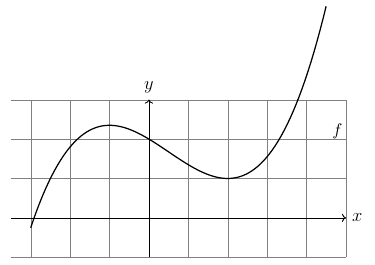
\includegraphics[width=0.6\linewidth]{data/calculus-figures/t3-b25-b26.png}\end{center}
\begin{list}{}{\setlength{\leftmargin}{3em}\setlength{\labelwidth}{2.5em}\setlength{\itemsep}{0pt}\setlength{\topsep}{2pt}}
\item[(A)] $0.3$
\item[(B)] $0.8$
\item[(C)] $1.2$
\item[(D)] $1.8$
\end{list}

\bigskip\noindent\textbf{TB26.}\ Use the graph below; each grid interval represents one unit. The rate of change of $f(x)$ is least at $x \approx$
\begin{center}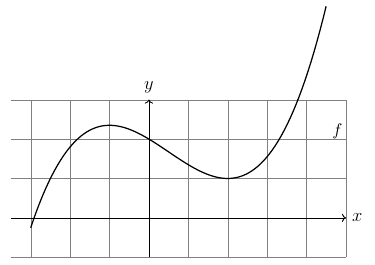
\includegraphics[width=0.6\linewidth]{data/calculus-figures/t3-b25-b26.png}\end{center}
\begin{list}{}{\setlength{\leftmargin}{3em}\setlength{\labelwidth}{2.5em}\setlength{\itemsep}{0pt}\setlength{\topsep}{2pt}}
\item[(A)] $-1$
\item[(B)] $0.5$
\item[(C)] $1.5$
\item[(D)] $3$
\end{list}

\bigskip\noindent\textbf{TB27.}\ For $f(x) = 3^x$, what is the estimate of $f'(2)$ obtained by using the symmetric difference quotient with $h=0.04$?
\begin{list}{}{\setlength{\leftmargin}{3em}\setlength{\labelwidth}{2.5em}\setlength{\itemsep}{0pt}\setlength{\topsep}{2pt}}
\item[(A)] $9.548$
\item[(B)] $9.891$
\item[(C)] $9.985$
\item[(D)] $19.775$
\end{list}

\bigskip\noindent\textbf{TB28.}\ To how many places is the symmetric difference quotient accurate when it is used to approximate $f'(0)$ for $f(x) = 6^x$ and $h = 0.05$?
\begin{list}{}{\setlength{\leftmargin}{3em}\setlength{\labelwidth}{2.5em}\setlength{\itemsep}{0pt}\setlength{\topsep}{2pt}}
\item[(A)] $1$
\item[(B)] $2$
\item[(C)] $3$
\item[(D)] more than 3
\end{list}

\bigskip\noindent\textbf{TB29.}\ For $f(x)=6^x$, to how many decimal places does the symmetric quotient $[f(h)-f(-h)]/(2h)$ with $h=0.001$ agree with $f\prime(0)$?
\begin{list}{}{\setlength{\leftmargin}{3em}\setlength{\labelwidth}{2.5em}\setlength{\itemsep}{0pt}\setlength{\topsep}{2pt}}
\item[(A)] $1$
\item[(B)] $2$
\item[(C)] $3$
\item[(D)] more than 3
\end{list}

\bigskip\noindent\textbf{TB30.}\ What numerical value does the symmetric difference quotient $[f(h)-f(-h)]/(2h)$ give for $f(x)=|x|$ with $h=0.0005$?
\begin{list}{}{\setlength{\leftmargin}{3em}\setlength{\labelwidth}{2.5em}\setlength{\itemsep}{0pt}\setlength{\topsep}{2pt}}
\item[(A)] $-1$
\item[(B)] $0$
\item[(C)] $1$
\item[(D)] indeterminate
\end{list}

\bigskip\noindent\textbf{TB31.}\ If $\dfrac{d}{dx}f(x) = g(x)$ and $h(x) = \cos x$, then $\dfrac{d}{dx}f(h(x))$ equals
\begin{list}{}{\setlength{\leftmargin}{3em}\setlength{\labelwidth}{2.5em}\setlength{\itemsep}{0pt}\setlength{\topsep}{2pt}}
\item[(A)] $g(\cos x)$
\item[(B)] $\cos x \cdot g(x)$
\item[(C)] $-\sin x \cdot g(\cos x)$
\item[(D)] $\sin x \cdot g(\cos x)$
\end{list}

\bigskip\noindent\textbf{TB32.}\ Let $f(x) = 2^x - x^2$. The tangent to the curve is parallel to the secant through $(0,1)$ and $(4,0)$ for $x =$
\begin{list}{}{\setlength{\leftmargin}{3em}\setlength{\labelwidth}{2.5em}\setlength{\itemsep}{0pt}\setlength{\topsep}{2pt}}
\item[(A)] $0.680$ only
\item[(B)] $3.103$ only
\item[(C)] $0.680$ and $3.103$ only
\item[(D)] no such value of $x$ exists
\end{list}

\bigskip\noindent\textbf{TB33.}\ On the interval $1<x<2$, $f(x)$ equals
\begin{center}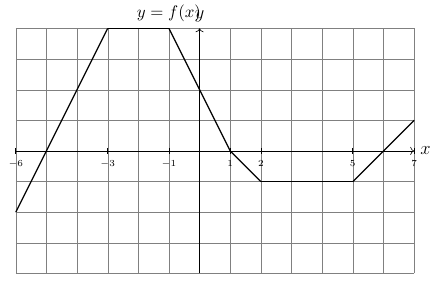
\includegraphics[width=0.6\linewidth]{data/calculus-figures/t3-b33-b37.png}\end{center}
\begin{list}{}{\setlength{\leftmargin}{3em}\setlength{\labelwidth}{2.5em}\setlength{\itemsep}{0pt}\setlength{\topsep}{2pt}}
\item[(A)] $-x-1$
\item[(B)] $-x+1$
\item[(C)] $-x-2$
\item[(D)] $-x+2$
\end{list}

\bigskip\noindent\textbf{TB34.}\ Over which of the following intervals does $f'(x)$ equal zero?

I. $(-6,-3)$
II. $(-3,-1)$
III. $(2,5)$
\begin{center}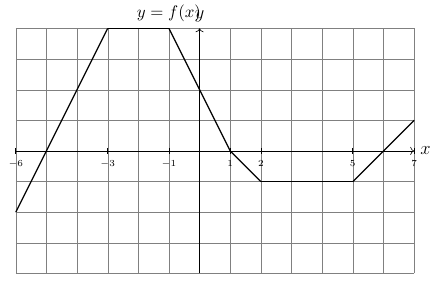
\includegraphics[width=0.6\linewidth]{data/calculus-figures/t3-b33-b37.png}\end{center}
\begin{list}{}{\setlength{\leftmargin}{3em}\setlength{\labelwidth}{2.5em}\setlength{\itemsep}{0pt}\setlength{\topsep}{2pt}}
\item[(A)] II only
\item[(B)] I and II only
\item[(C)] I and III only
\item[(D)] II and III only
\end{list}

\bigskip\noindent\textbf{TB35.}\ How many points of discontinuity does $f'(x)$ have on the interval $-6<x<7$?
\begin{center}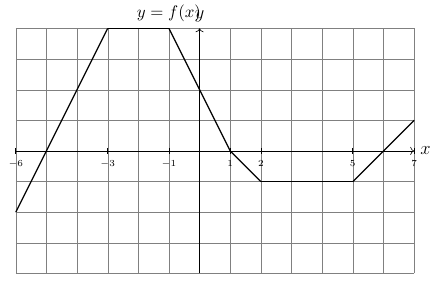
\includegraphics[width=0.6\linewidth]{data/calculus-figures/t3-b33-b37.png}\end{center}
\begin{list}{}{\setlength{\leftmargin}{3em}\setlength{\labelwidth}{2.5em}\setlength{\itemsep}{0pt}\setlength{\topsep}{2pt}}
\item[(A)] $2$
\item[(B)] $3$
\item[(C)] $4$
\item[(D)] $5$
\end{list}

\bigskip\noindent\textbf{TB36.}\ For $-6<x<-3$, $f'(x)$ equals
\begin{center}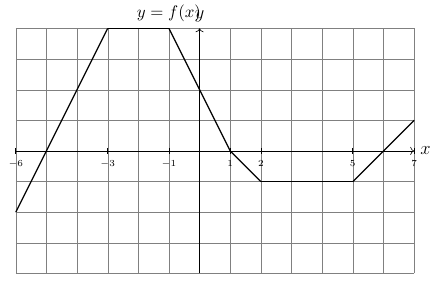
\includegraphics[width=0.6\linewidth]{data/calculus-figures/t3-b33-b37.png}\end{center}
\begin{list}{}{\setlength{\leftmargin}{3em}\setlength{\labelwidth}{2.5em}\setlength{\itemsep}{0pt}\setlength{\topsep}{2pt}}
\item[(A)] $-2$
\item[(B)] $-1$
\item[(C)] $1$
\item[(D)] $2$
\end{list}

\bigskip\noindent\textbf{TB37.}\ Which of the following statements about the graph of $f'(x)$ is false?
\begin{center}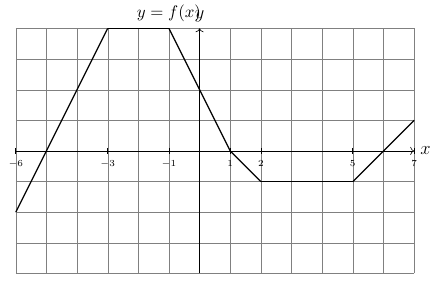
\includegraphics[width=0.6\linewidth]{data/calculus-figures/t3-b33-b37.png}\end{center}
\begin{list}{}{\setlength{\leftmargin}{3em}\setlength{\labelwidth}{2.5em}\setlength{\itemsep}{0pt}\setlength{\topsep}{2pt}}
\item[(A)] $f'(x)$ consists of six horizontal segments
\item[(B)] $f'(x)$ has four jump discontinuities
\item[(C)] $f'(x)$ is discontinuous at each $x$ in the set $\{-3,-1,1,2,5\}$
\item[(D)] On the interval $-1<x<1$, $f'(x) = -2$
\end{list}

\bigskip\noindent\textbf{TB38.}\ The table gives the values of a function $f$ that is differentiable on the interval $[0,1]$:

\[\begin{array}{|c|c|c|c|c|c|c|}
\hline
x & 0.15 & 0.25 & 0.31 & 0.45 & 0.57 & 0.65 \\
\hline
f(x) & 0.200 & 0.310 & 0.375 & 0.402 & 0.390 & 0.350 \\
\hline
\end{array}\]

According to this table, the best approximation of $f'(0.15)$ is
\begin{list}{}{\setlength{\leftmargin}{3em}\setlength{\labelwidth}{2.5em}\setlength{\itemsep}{0pt}\setlength{\topsep}{2pt}}
\item[(A)] $0.11$
\item[(B)] $1.03$
\item[(C)] $1.10$
\item[(D)] $1.75$
\end{list}

\bigskip\noindent\textbf{TB39.}\ Let $f(x) = x^3-6x^2+9x$ on $[0,5]$. At how many points in $(0,5)$ does $f$ satisfy the conclusion of the Mean Value Theorem?
\begin{list}{}{\setlength{\leftmargin}{3em}\setlength{\labelwidth}{2.5em}\setlength{\itemsep}{0pt}\setlength{\topsep}{2pt}}
\item[(A)] none
\item[(B)] $1$
\item[(C)] $2$
\item[(D)] $3$
\end{list}

\end{document}
